%----------------------------------------------------------------------------------------
%	Inställningar och dokumentkonfiguration
%----------------------------------------------------------------------------------------

\documentclass[paper=a4, fontsize=11pt]{report} % A4-sida och 11 punkters fontstorlek

\usepackage[T1]{fontenc} % 8-bitarskodning som har 256 glyfer
\usepackage[swedish]{babel} % Svenskt språk
\usepackage[utf8]{inputenc} % För svenska tecken
\usepackage{dtklogos} % Logos
\usepackage{wallpaper} % Bakgrundsbild
\usepackage{fancyhdr} % Specialsidhuvud och sidfot
\usepackage{enumerate} 
\usepackage{xifthen}% provides \isempty test
\usepackage{listings}% Code examples
\usepackage{xcolor}

\lstdefinestyle{BashInputStyle}{
  language=bash,
  basicstyle=\small\sffamily,
  numbers=left,
  numberstyle=\tiny,
  numbersep=3pt,
  frame=tb,
  columns=fullflexible,
  backgroundcolor=\color{yellow!20},
  linewidth=0.9\linewidth,
  xleftmargin=0.1\linewidth
}
% Exampels
% Inline
% \lstinline[style=BashInputStyle]´# apt-get --purge remove rubygems´.
% Multiline
% \begin{lstlisting}[style=BashInputStyle]
%    # apt-get --purge remove rubygems
% \end{lstlisting}

\pagestyle{fancyplain} % Använd sidhuvud och sidfot på alla sidor
\fancyhead[L]{Seminar 2 -- 1DV020 -- 2015 -- Server Administration} % Titel till vänster i sidhuvud
\fancyhead[C]{} % Tomt i mitten
\fancyhead[R]{} % Tomt till höger
\fancyfoot[L]{} % Tomt till vänster
\fancyfoot[C]{} % Tomt i mitten
\fancyfoot[R]{\thepage} % Sidnumrering till höger i sidfoten
\renewcommand\thesection{\arabic{section}} % Section beter sig som i dokumentklassen article

\newcommand{\win}[1]{Microsoft Windows Server\ifthenelse{\isempty{#1}}{}{ #1}}
\newcommand{\gui}[0]{``Server with a GUI''}
\newcommand{\core}[0]{Windows Server Core}
%----------------------------------------------------------------------------------------
%	TITLE SECTION
%----------------------------------------------------------------------------------------
\newcommand\BackgroundPic{
    \put(-50,-50){
    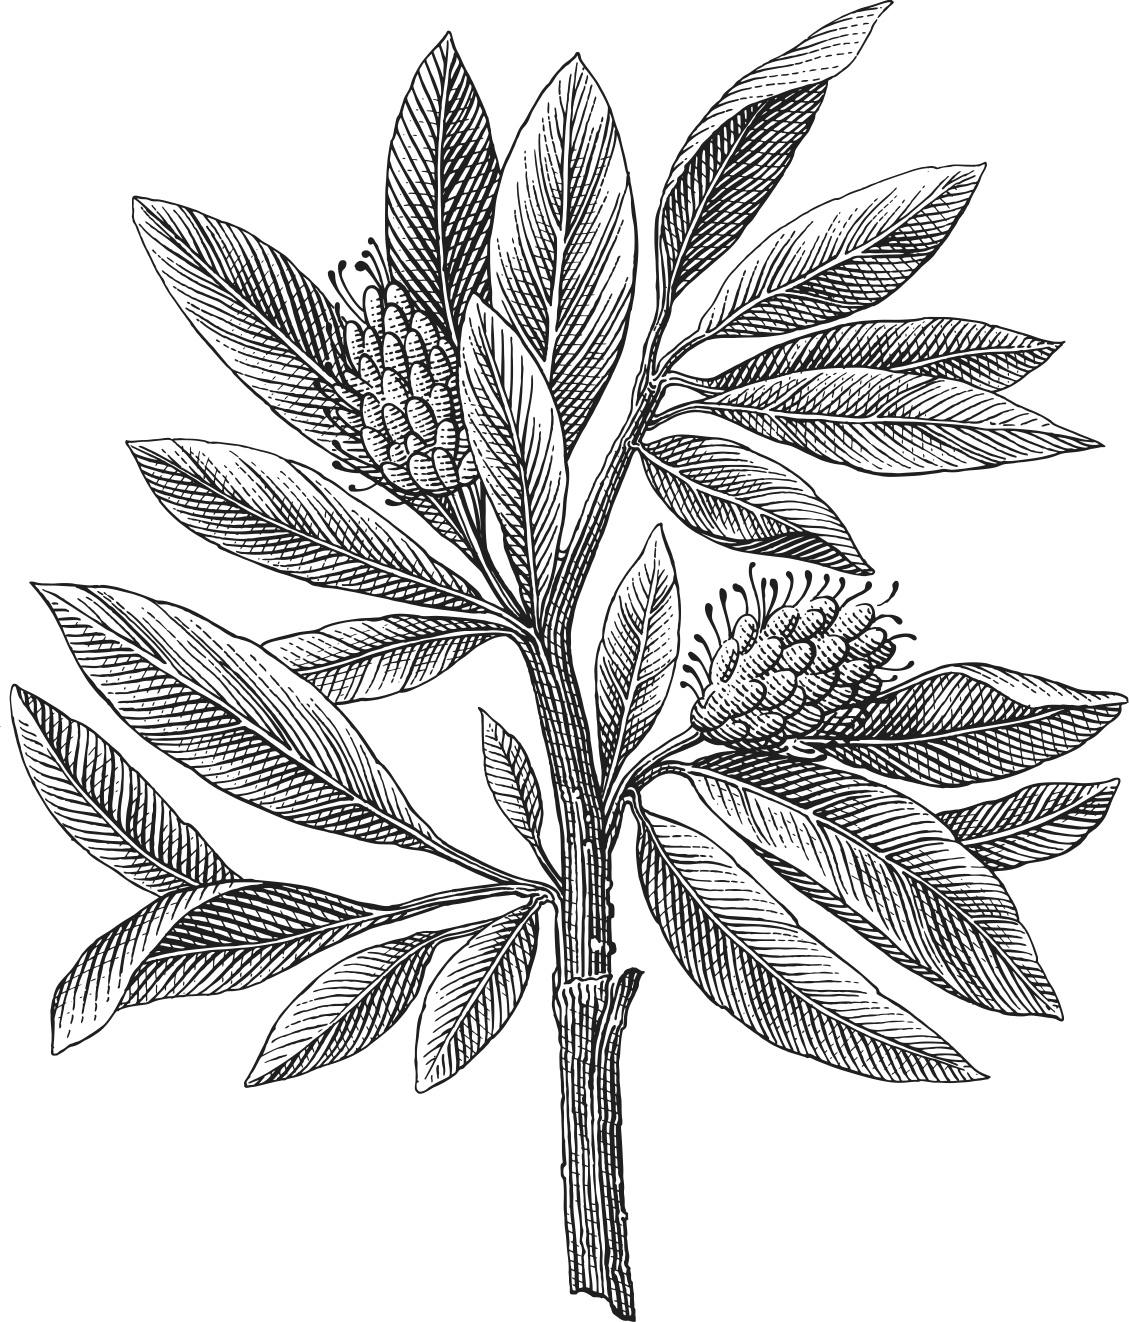
\includegraphics[keepaspectratio,scale=0.65]{lnu_etch.png} % Bakgrundsbild
    }
}
\newcommand\BackgroundPicLogo{
    \put(15,700){
    
\includegraphics[keepaspectratio,scale=0.10]{logo.png} % Logga i vänstra hörnet
    }
}

\newcommand{\horrule}[1]{\rule{\linewidth}{#1}} % Skapa hortisontell linje

\title{	\vspace{-10cm}
    \normalfont \normalsize
    \textsc{Linnaeus University} \\ [25pt] % Universitetes namn
    \horrule{0.5pt} \\[0.4cm] % Tunn linje högst upp
    \huge Seminar 2\\ % Arbetes titel
	\large \textcolor{gray}{1DV020 -- Server Administration}
    \horrule{0.5pt} \\[0.4cm] % Tunn linje längst ner
}

\author{Jacob Lindehoff} % Författarnas namn

\date{\normalsize\today} % Dagens datum

\begin{document}
  \AddToShipoutPicture*{\BackgroundPic} % Lägger in backgrundsbild på första sidan
  \AddToShipoutPicture*{\BackgroundPicLogo}
  \maketitle % Skriv ut titeln
  \noindent % Tabba inte in på första meningen

  %------------------------------------------------
  % Introduktion
  %------------------------------------------------
  \section{Introduction}
  During this seminar, we will address the following topics:
  \begin{itemize}
    \item File Systems: NTFS, EXT
    \item Local Users and Groups
    \item Storage – RAID
    \item File server - SMB and Samba
  \end{itemize}

  %------------------------------------------------
  %	Deadline
  %------------------------------------------------
  \section{Deadline}
  The seminar is on the {\color{red}11th of February 2015} and it is compulsory. If you cannot participate, it must be notified in advance and a written report of the seminar must be submitted no later than {\color{red}3 days} after the seminar. The written report should contain detailed answers to all questions in the seminar.
  \newpage

  %------------------------------------------------
  %	Seminariefrågor
  %------------------------------------------------
  \section{Seminar Questions}
  \subsection{File Systems}
  \begin{enumerate}
    \begin{large}
      \item Vilken extra funktionalitet får du med NTFS jämnfört med FAT32?
      \item Förklara hur rättighetsarv fungerar i NTFS?
      \item Vad är en ACL och vad innehåller den?
      \item Vad menas med kumulativa rättigheter?
      \item Vad händer med NTFS-rättigheterna när du
      \begin{enumerate}[a.]
      	\item flyttar en fil inom samma volym
      	\item kopierar en fil inom samma volym
      	\item flyttar en fil till en annan volym
      	\item kopierar en fil till en annan volym
      \end{enumerate}
      \item Kan mer än en användare vara ägare av en fil eller katalog, motivera ditt svar?
      \item Vilka är skillnaderna på NTFS-rättigheter och Utdelnings-rättigheter?
      \begin{enumerate}[a.]
      	\item Varför finns utdelningsrättigheter när vi kan använda NTFS-rättigheter istället?
      \end{enumerate}
      \item På vilka två sätt kan Windows hantera feltolerant disklagring?
      \item Förklara följande disklagringsmetoder, både hur de fungerar och när det rekommenderas att använda:
      \begin{enumerate}[a.]
      	\item Simple
      	\item Spanned
      	\item Striped
      	\item Mirrored
      	\item RAID-5
      \end{enumerate}
      \item Vad menas med NTFS-monterade enheter?
      \item Har NTFS stöd för Symboliska länkar som finns i t ex Linux?
      \setcounter{tmpc}{\theenumi}
    \end{large}
  \end{enumerate}

    \subsection{Access Control}
    \begin{enumerate}
    \setcounter{enumi}{\thetmpc}
    \begin{large}
    \item Vad är A G/U DL P strategin, beskriv i detalj och gärna med några exempel?
    \setcounter{tmpc}{\theenumi}
    \end{large}
  \end{enumerate}

\end{document}
